\documentclass[11pt]{exam}
\usepackage[margin=1in]{geometry}
\pagestyle{plain}
\usepackage{amsmath,amsfonts,amssymb,amsthm,enumerate}
\usepackage{multicol}
\usepackage[]{graphicx}
\usepackage{hyperref}
\usepackage{tikz}
\usepackage{pgfplots}
\usepackage{subfigure}
\usepackage[final]{pdfpages}

\everymath{\displaystyle}

\addtolength{\footskip}{2\baselineskip} % to lower the page numbers
\title{\vspace{-0.5in} Math 115 \\ Worksheet Section 5.2}
\date{}


% \theoremstyle{definition}
% \newtheorem{problem}{Problem}
\renewcommand{\questionlabel}{\textbf{Problem~\thequestion.}}
%\printanswers

\begin{document}
\maketitle
\vspace{-0.75in}
\begin{questions}
  \question Find the integral \[\int_0^{10} x-5 \,\:dx\] by finding the area of the region between the curve and the horizontal axis.
    \begin{solution}
      If we graph \(f(x) = x-5\), we see that \(\int_0^{10} x-5 dx =
      -12.5+12.5 = 0\).

      \begin{center}
        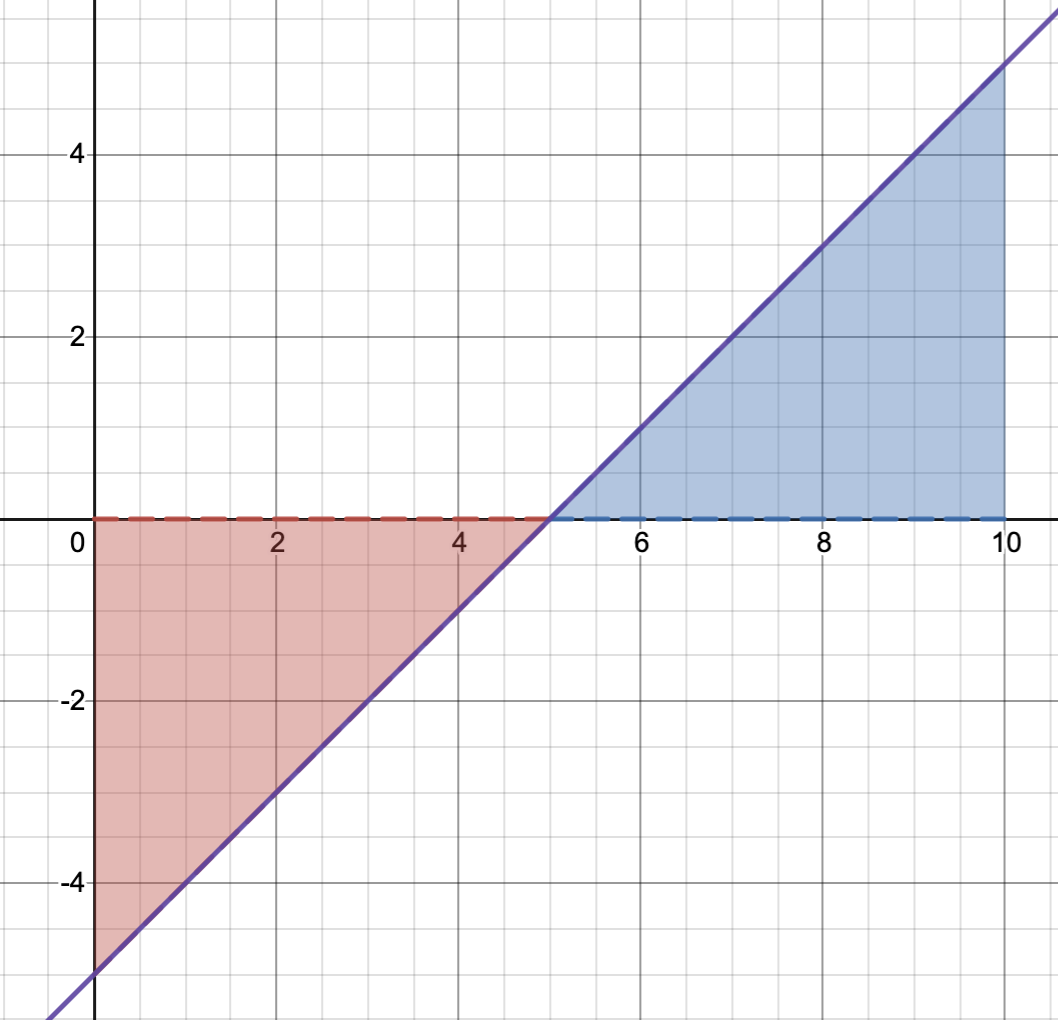
\includegraphics[scale=0.4]{Figures/s1}
      \end{center}
    \end{solution}
  \question Consider the function
\[
f(x) = \begin{cases}
1-x,	& 0 \leqslant x \leqslant 1,\\
x-1,	& 1 < x \leqslant 2.
\end{cases}
\]
\vspace{-2.5em}
\begin{enumerate}[(a)]
	\item Sketch the graph of $f$.
	\item Find $\displaystyle\int_0^2 f(x)\: dx$.
	\item Find the 4-term left Riemann sum approximation of the definite integral you just computed. How does your approximation compare to the exact value?
\end{enumerate}
\begin{solution}
  \begin{enumerate}[(a)]
  \item 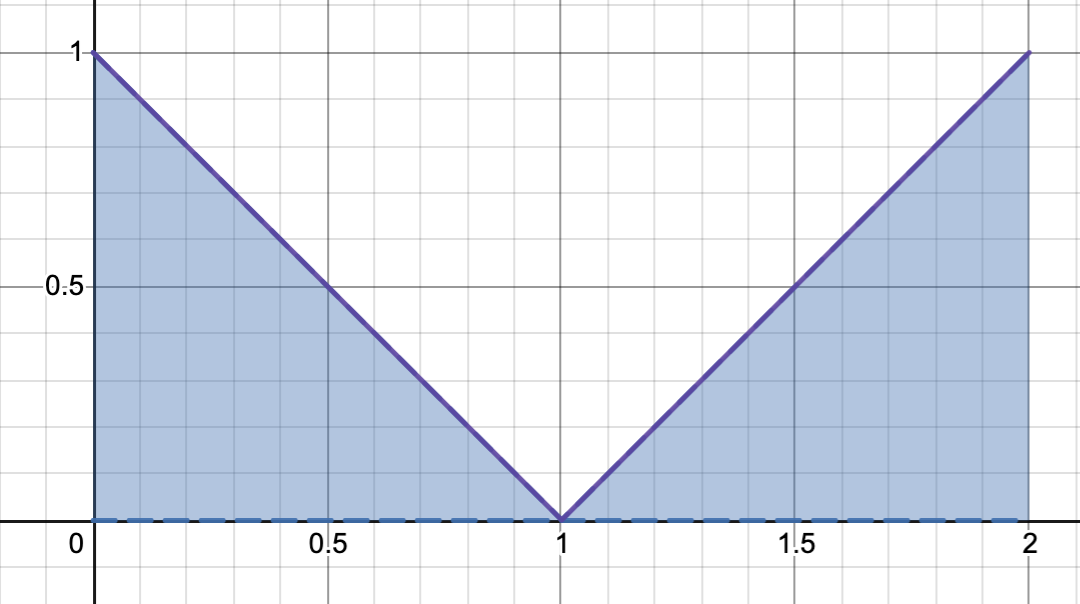
\includegraphics[scale=0.3]{Figures/s2}
  \item \(\int_0^2 f(x) dx = \frac{1}{2} + \frac{1}{2} = 1\)
  \item With \(n=4\), we get right-hand sum approximation \[
      0.5(0.5+0+0.5+1) = 1
    \]
  The left-hand sum approximation would be the same by symmetry. In
  this case, they are equal to the correct value.
  \end{enumerate}
\end{solution}
\question The plot below shows $y=g(x)$.
  \begin{center}
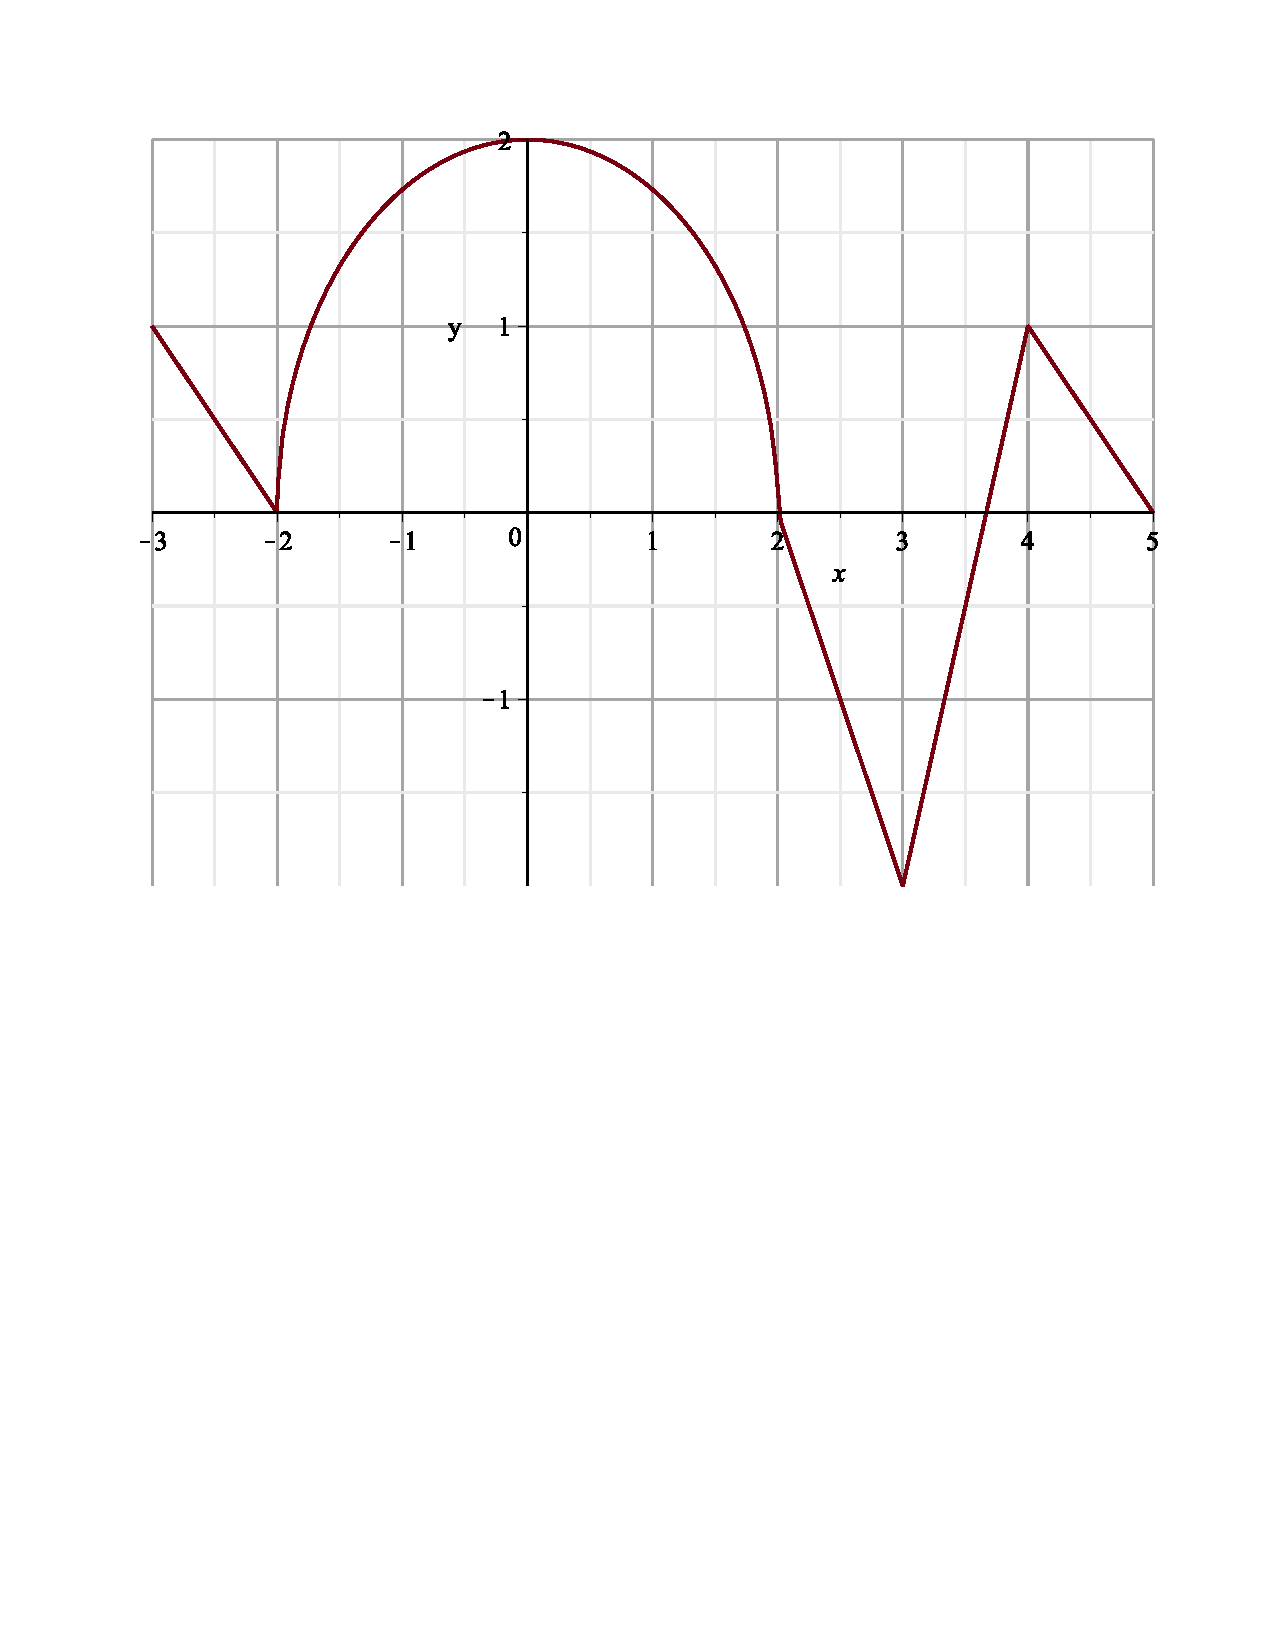
\includegraphics[width=11cm,height=5cm]{Figures/fig2.pdf}
  \end{center}
Find the exact value of
\begin{multicols}{2}
\begin{enumerate}[(a)]
	\item The definite integral $\displaystyle\int_{-3}^5g(x)\,dx$.
	\item The definite integral $\displaystyle\int_{-3}^5|g(x)|\,d x$.
\end{enumerate}
\end{multicols}
\begin{solution}
  \begin{enumerate}[(a)]
  \item We compute \[
      \int_{-3}^5 g(x) dx = \frac{1}{2}(1 \cdot 1) + \frac{1}{2} \pi
      2^2 + \frac{1}{2}(1)(-2) + \frac{1}{2}\left( \frac{2}{3}(-2)
      \right) + \frac{1}{2}\left( \frac{1}{3}(1) \right) + \frac{1}{2}(1)(1)
    \]
    % Thus, \(\int_{-3}^5 g(x) dx = 2\pi-\frac{5}{8}\).
  \item \[
      \int_{-3}^5 |g(x)| dx =  \frac{1}{2}(1 \cdot 1) + \frac{1}{2} \pi
      2^2 + \frac{1}{2}(1)(2) + \frac{1}{2}\left( \frac{2}{3}(2)
      \right) + \frac{1}{2}\left( \frac{1}{3}(1) \right) + \frac{1}{2}(1)(1)
    \]
    % Thus, \(\int_{-3}^5 |g(x)| dx = 2\pi + \frac{19}{8}\).
  \end{enumerate}
\end{solution}
\question Use the figure below to compute the values of 
  \begin{multicols}{2}
    \begin{enumerate}[(a)]
    \item \(\int_a^b f(x) dx\)
    \item \(\int_b^c f(x) dx\)
    \item \(\int_a^c f(x) dx\)
    \item \(\int_a^c |f(x)| dx\)
    \end{enumerate}
    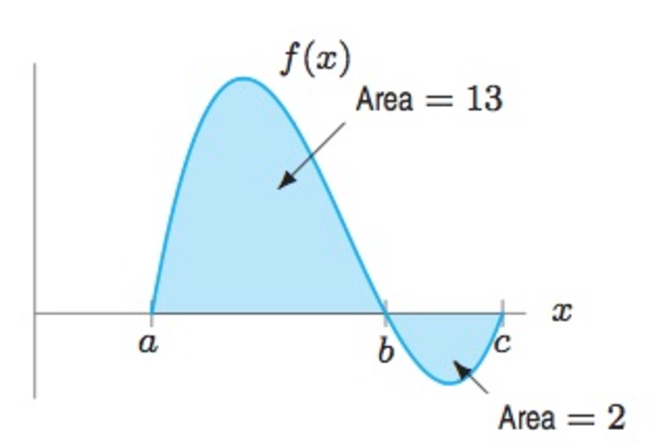
\includegraphics[scale=0.5]{Figures/no29graph.pdf}
  \end{multicols}
  \begin{solution}
    \begin{enumerate}[(a)]
    \item \(13\)
    \item \(-2\)
    \item \(11\)
    \item \(15\)
    \end{enumerate}
  \end{solution}
\question (Fall 2016 Final Exam) % Problem 1
	A portion of the graph of a function $f$ is shown below.
        \begin{center}
		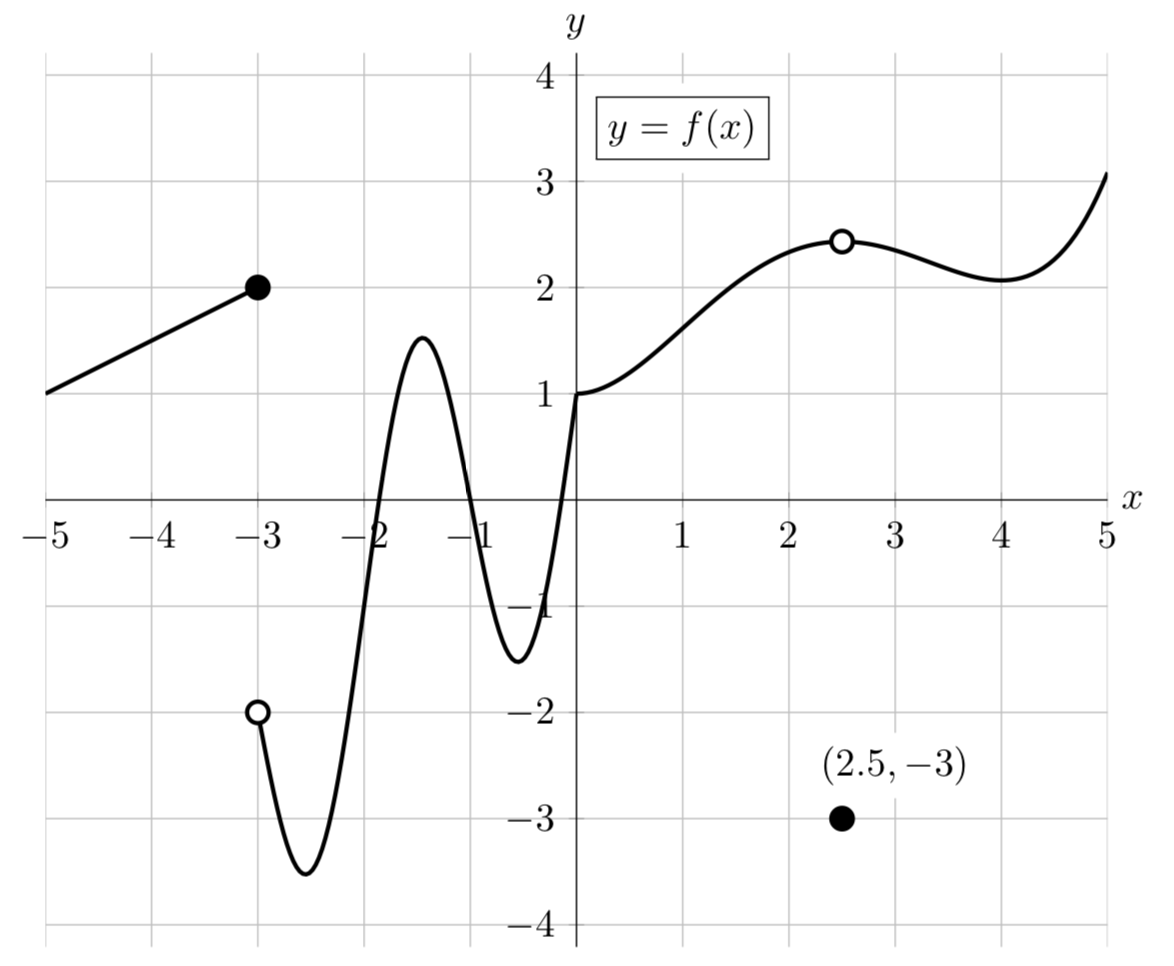
\includegraphics[scale=0.5]{Figures/graphf}
        \end{center}
	\begin{enumerate}[(a)]
		\item For which of the values of $c$ is $\lim_{x \rightarrow c^-} f(x) = f(c)$?
		$$c=-3 \hspace{3em} c=-1 \hspace{3em} c=0 \hspace{3em} c=1 \hspace{3em} c=2.5 \hspace{3em} \textrm{none}$$
		\item For which of the following values of $c$ is $f(x)$ continuous at $x=c$?
		$$c=-3 \hspace{3em} c=-1 \hspace{3em} c=0 \hspace{3em} c=1 \hspace{3em} c=2.5 \hspace{3em} \textrm{none}$$
		\item For which of the following values of $c$ does $f$ appear to be differentiable at $x=c$?
		$$c=-3 \hspace{3em} c=-1 \hspace{3em} c=0 \hspace{3em} c=1 \hspace{3em} c=2.5 \hspace{3em} \textrm{none}$$
		\item Rank the following quantities in order from least to greatest:
		\begin{enumerate}[I.]
		\item The number $0$.
		\item $f(1)$.
		\item $\displaystyle\int_{-1}^1 f(x) dx$.
		\item The left-hand Riemann sum with 2 subintervals for $\displaystyle\int_{-1}^1 f(x) dx$.
		\item The right-hand Riemann sum with 2 subintervals for $\displaystyle\int_{-1}^1 f(x) dx$.
		\end{enumerate}
	\end{enumerate}
        \begin{solution}
          See \href{https://dhsp.math.lsa.umich.edu/exams/115exam3/f16/s1.pdf}{https://dhsp.math.lsa.umich.edu/exams/115exam3/f16/s1.pdf}
        \end{solution}
        \pagebreak
\question We want to compute $\displaystyle\int_0^2 \sqrt{t} \, dt$. Below is a portion of the graph of $f(t)=\sqrt{t}$.
  \begin{center}
    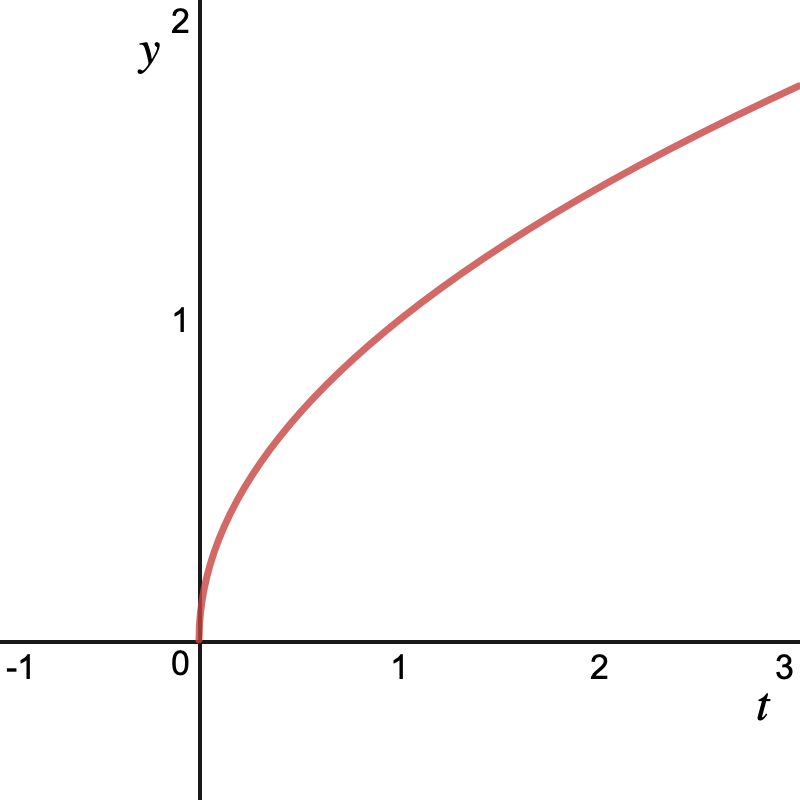
\includegraphics[scale=.2]{Figures/sqrt}
  \end{center}
\begin{enumerate}[(a)]
	\item For this integral, are left sums always overestimates, always underestimates, or could they be either? What about right sums?
	\item Use a Riemann sum with $5$ equal subdivisions to find a lower estimate for the integral. Show your answer to three decimal places.
	\item Use a Riemann sum with $5$ equal subdivisions to find an upper estimate for the integral. Show your answer to three decimal places.
	\item Repeat (b) and (c) with $10$ equal subdivisions. Show your answers to three decimal places.
\end{enumerate}
\begin{solution}
  \begin{enumerate}[(a)]
  \item Left sums will always be underestimates
  \item \[
      \frac{2}{5}\left( 0+\sqrt{2/5}+\sqrt{4/5}+\sqrt{6/5}+\sqrt{8/5}
      \right) \approx 1.555
    \]
  \item \[
      \frac{2}{5}\left( \sqrt{2/5}+\sqrt{4/5}+\sqrt{6/5}+\sqrt{8/5} +
        \sqrt{2} \right) \approx 2.121
    \]
  \item With the 10 equal subdivisions, the left-hand sum is \(1.727\)
    and the right-hand sum is \(2.010\). 
  \end{enumerate}
\end{solution}
\question For each of the following statements, must the statement be true for all continuous functions $f(x)$ and $g(x)$? Explain your answer.
\begin{enumerate}[(a)]
	\item $\displaystyle\int_0^2 f(x) \: dx \leqslant \displaystyle\int_0^3 f(x)\: dx$.
	\item $\displaystyle\int_0^2 f(x) \: dx = \displaystyle\int_0^2 f(t)\: dt$.
	\item If $\displaystyle\int_2^6 f(x) \: dx \leqslant \int_2^6 g(x)\: dx$, then $f(x) \leqslant g(x)$ for all $2 \leqslant x \leqslant 6$.	
\end{enumerate}
\begin{solution}
  \begin{enumerate}[(a)]
  \item No. Consider \(f(x) = -1\). 
  \item Yes. It is irrelevant what you call the integrated variable.
  \item No. Consider \(f(x) = x-4\) and \(g(x) = 1\). 
  \end{enumerate}
\end{solution}
\question Sketch the graph of a function \(f\) (you do not need to
  give a formula for \(f\)) on an interval \([a,b]\) with the property
  that with \(n=2\) subdivisions, \[
    \int_a^b f(x) dx < \text{ Left-hand sum } < \text{ Right-hand sum.}
  \]
  \begin{solution}
    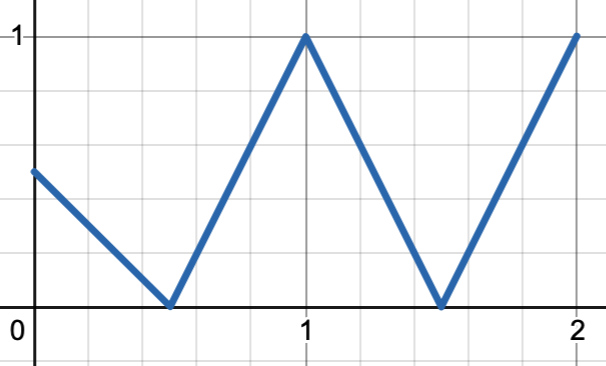
\includegraphics[scale=0.5]{Figures/s8.png} with \(a=0\) and \(b=2\).
  \end{solution}
\question Without computing the sums, find the difference between the
  right- and left-hand Riemann sums if we use \(n=500\) subintervals
  to approximate \(\int_{-1}^1 (2x^3+4) dx\).
  \begin{solution}
    For \(f(x) = 2x^3+4\), the difference (with possible sign) will be
    \(\frac{1}{500}(f(b)-f(a))\) for \(b = -1\) and \(a=1\). This
    gives \[
      \frac{1}{500}(-2+4-(2+4)) =
      \frac{1}{500}(-4) = -\frac{1}{125}
    \]
    So, the two estimates differ by \(\frac{1}{125}\).
  \end{solution}
\question Compute the following integrals by interpreting them in
  terms of area.
  \vspace{-0.25cm}
  \begin{multicols}{3}
    \begin{enumerate}[(a)]
    \item \(\int_{-1}^2 |x-1| dx\)
    \item \(\int_0^1 \sqrt{1-x^2} dx\)
    \item \(\int_{-\pi}^\pi \sin(x) dx\)
    \end{enumerate}
  \end{multicols}
  \begin{solution}
    \begin{enumerate}[(a)]
    \item We draw the following graph.

     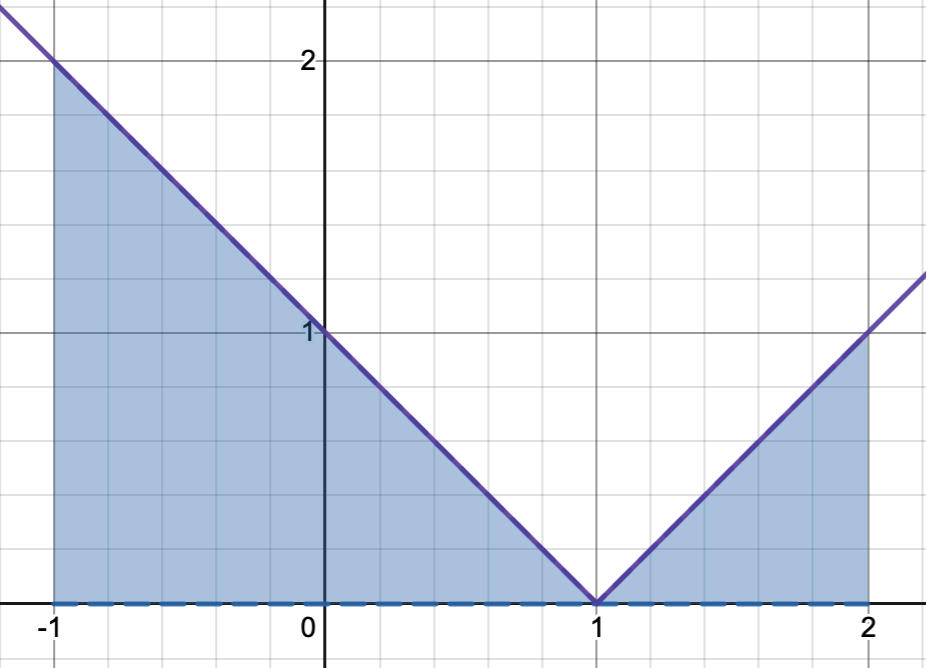
\includegraphics[scale=0.5]{Figures/s10a}

     From this, we conclude \(\int_{-1}^2 |x-1| dx =
     \frac{1}{2}(2\cdot 2 + 1 \cdot 1) = \frac{5}{2}\).
    \item We draw the following graph.

    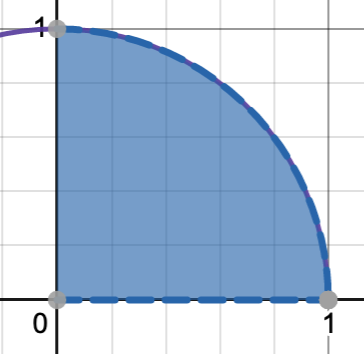
\includegraphics[scale=0.5]{Figures/s10b}

    From this, we see we need the area of a quarter circle of radius
    1, so \(\int_0^1 \sqrt{1-x^2} dx = \frac{\pi}{4}\)
    \item We draw the following graph.

    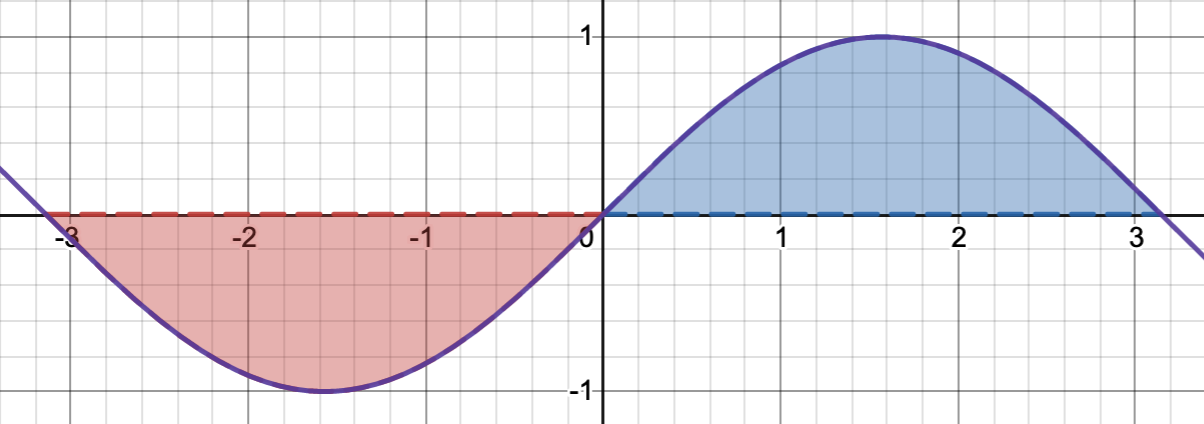
\includegraphics[scale=0.5]{Figures/s10c}

    From this, we see the answer is 0, which makes sense since
    \(\sin\) is an odd function.
    \end{enumerate}
  \end{solution}
\question Give an example of a function \(f\) such that \(\int_1^3
  f(x) dx < \int_1^2 f(x) dx\).
  \begin{solution}
   Consider \(f(x) = -1\). 
  \end{solution}
\question Decide whether the following statement is true or false and
  justify your answer.
  \begin{parts}
  \part On the interval \(a \leq t \leq b\), the integral of the
    velocity is the total distance traveled from \(t=a\) to \(t=b\).
  \part A 4-term left-hand Riemann sum approximation cannot give the
    exact value of a definite integral.
  \part If \(f(x)\) is decreasing and \(g(x)\) is increasing, then
    \(\int_a^b f(x) dx \neq \int_a^b g(x) dx\).
  \end{parts}
  \begin{solution}
    \begin{enumerate}[(a)]
    \item False. The integral of the velocity is the total displacement.
    \item False. This can happen in special cases. For instance, if
      you take the definite integral of a constant function.
    \item False. \[
        \int_0^1 x dx = \int_0^1 (1-x) dx
      \] 
    \end{enumerate}
  \end{solution}
\question Graph a continuous function \(f(x) \geq 0\) on \([0,10]\)
  with the given properties.
  \begin{parts}
  \part The maximum value taken on by \(f(x)\) for \(0 \leq x \leq
    10\) is \(1\). In addition, \(\int_0^{10} f(x) dx = 5\). 
  \part The maximum value taken on by \(f(x)\) for \(0 \leq x \leq
    10\) is \(5\). In addition, \(\int_0^{10} f(x) dx = 1\). 
  \end{parts}
  \begin{solution}
    \begin{enumerate}[(a)]
    \item 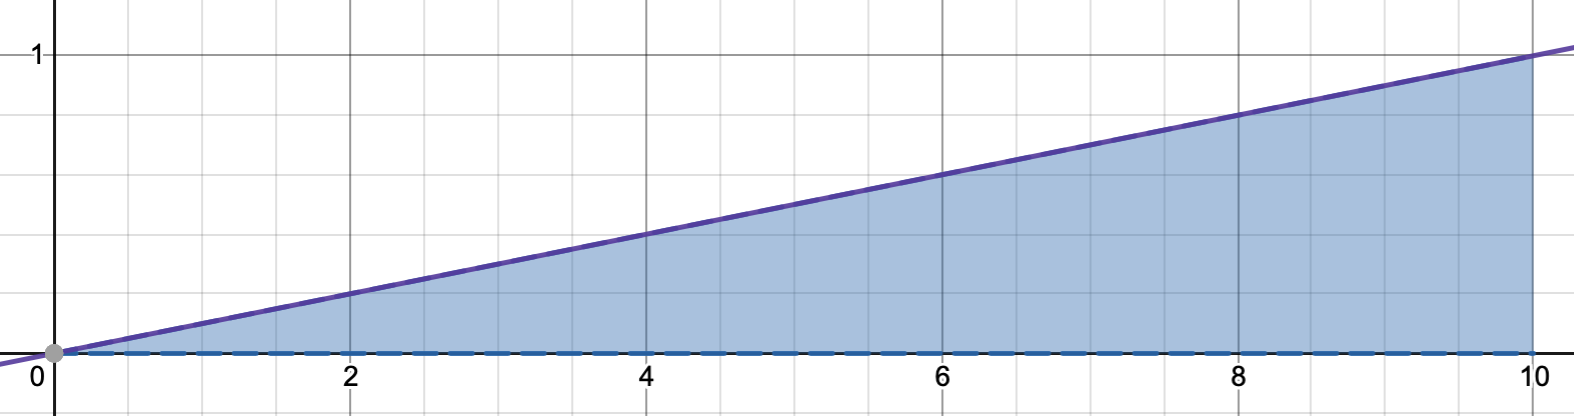
\includegraphics[scale=0.5]{Figures/s13a}
    \item 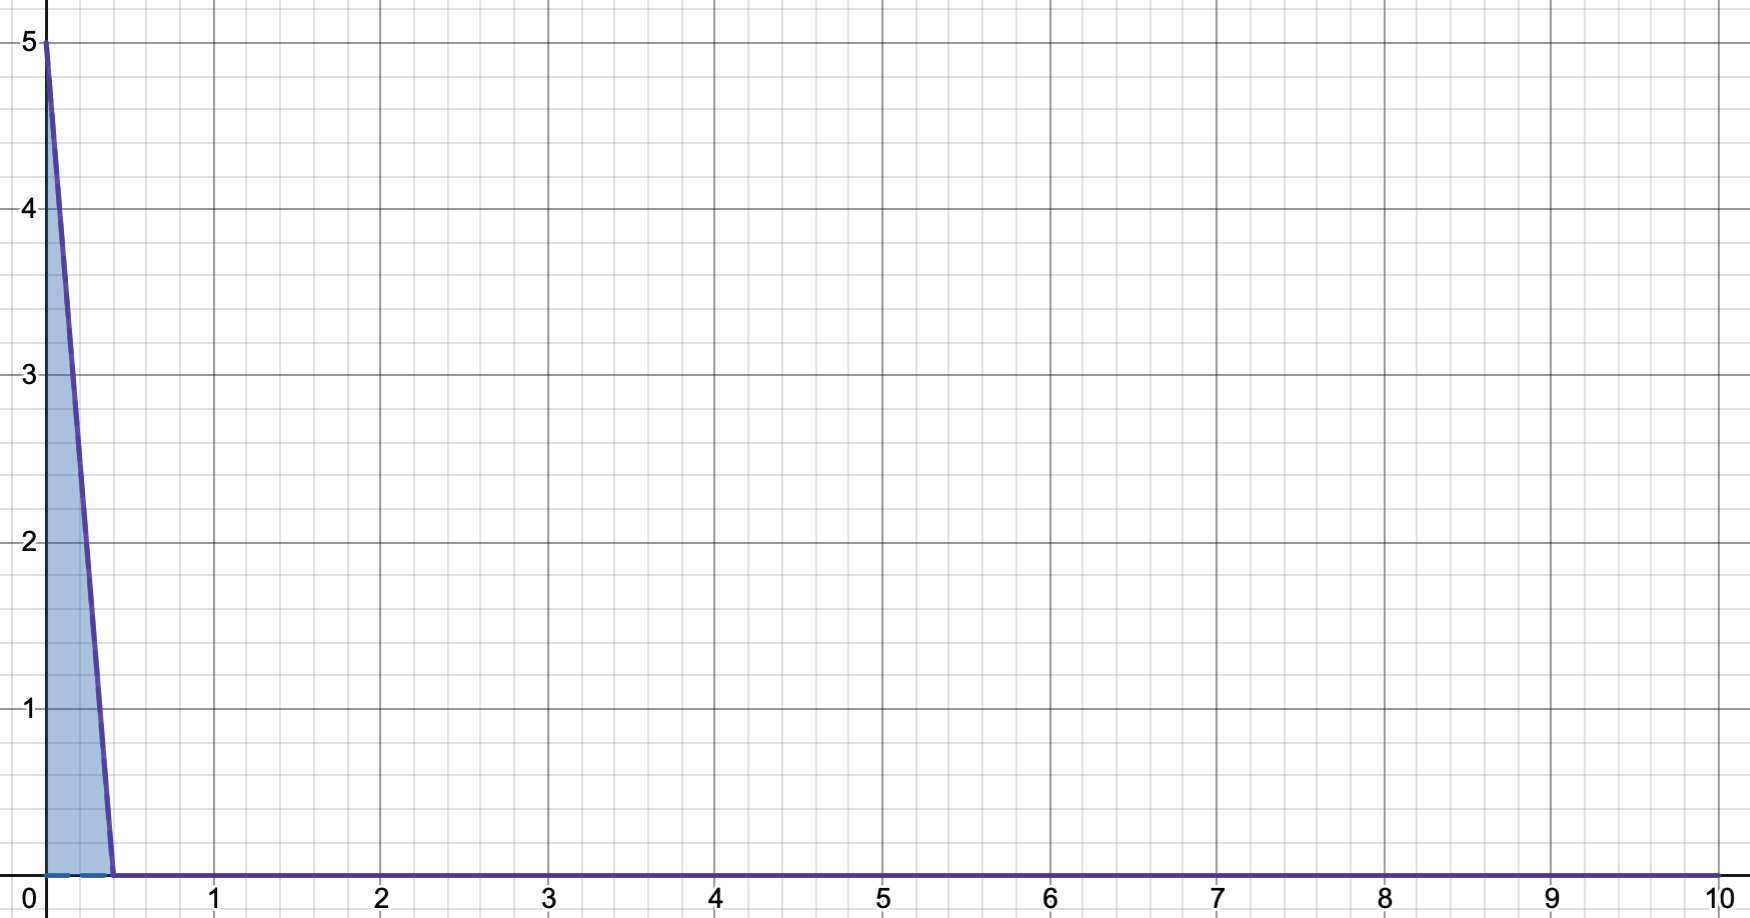
\includegraphics[scale=0.5]{Figures/s13b}
    \end{enumerate}
  \end{solution}
\question Use the figure to find limit \(a\) and \(b\) in the interval
  \([0,5]\) with \(a<b\) satisfying the given condition.
  \begin{multicols}{2}
    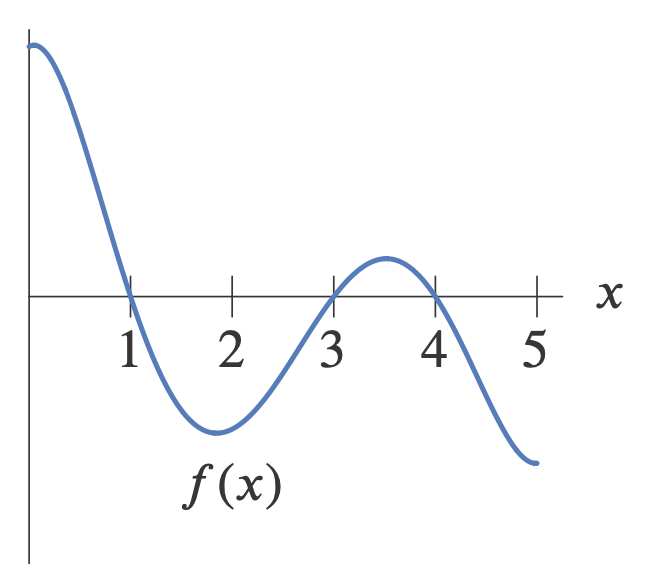
\includegraphics[scale=0.5]{Figures/graph14}
    \begin{parts}
    \part \(\int_0^b f(x) dx\) is as large as possible.
    \part \(\int_a^4 f(x) dx\) is as small as possible.
    \part \(\int_a^b f(x) dx\) is as large as possible.
    \part \(\int_a^b f(x) dx\) is as small as possible.
    \end{parts}
  \end{multicols}
  \begin{solution}
    \begin{enumerate}[(a)]
    \item \(b=1\)
    \item \(a=3\)
    \item \(a=0\), \(b=1\)
    \item \(a=1\), \(b=5\)
    \end{enumerate}
  \end{solution}
\end{questions}
\end{document}
%%% Local Variables:
%%% mode: latex
%%% TeX-master: t
%%% End:
